\documentclass[a4paper,11pt]{beamer}

\usepackage{../préambule-beamer}
\usetikzlibrary{positioning}

\title{Correction exercice 48 page 194}
\date{10 novembre}
\author{}

\begin{luacode}
	dofile "symetrie.lua"
\end{luacode}

\begin{document}

\begin{frame}
	\begin{center}
		\LARGE
		\myuline{Correction exercice 48 page 194}
		\vspace{1em}
	\end{center}
\end{frame}

\newcommand{\myfigurescale}{0.6}

\begin{frame}
	\begin{center}
		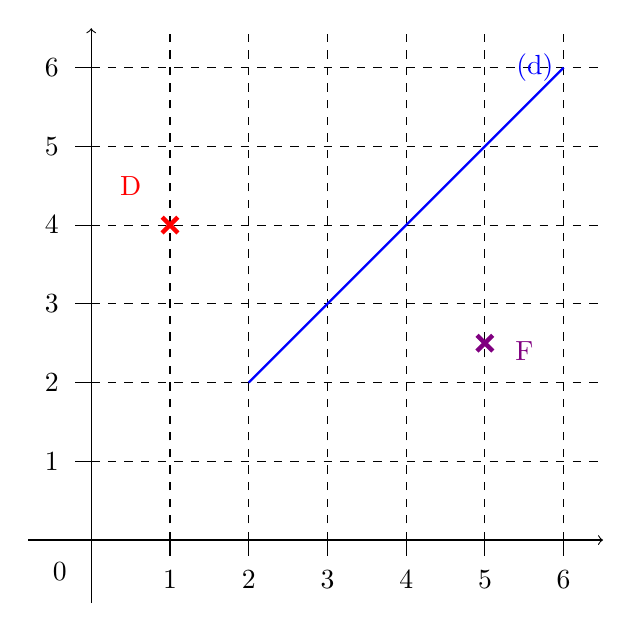
\begin{tikzpicture}
			\draw[dashed] (0,0) grid (6.5,6.5);
			\draw[->] (-0.8,0) -- (6.5,0);
			\draw[->] (0,-0.8) -- (0,6.5);
			\node at (-0.4,-0.4) {0};
			\foreach \r in {1,...,6}{
					\draw (\r,0) -- (\r,-0.2);
					\node at (\r,-0.5) {\r};

					\draw (0,\r) -- (-0.2,\r);
					\node at (-0.5,\r) {\r};
				}

			\coordinate (Dpoint) at (1,4);
			\draw[red,ultra thick] (Dpoint) ++(-0.1,-0.1) -- ++(0.2,0.2) ++(-0.2,0) -- ++(0.2,-0.2);
			\node[red] at ([yshift=0.5cm,xshift=-0.5cm] Dpoint) {D};

			\draw[blue,thick] (2,2) -- (6,6) node[anchor=east] {(d)};

			\coordinate (Fpoint) at (5,2.5);
			\draw[violet,ultra thick] (Fpoint) ++(-0.1,-0.1) -- ++(0.2,0.2) ++(-0.2,0) -- ++(0.2,-0.2);
			\node[violet] at ([yshift=-0.1cm,xshift=0.5cm] Fpoint) {F};
		\end{tikzpicture}
	\end{center}
\end{frame}

\begin{frame}
	\begin{center}
		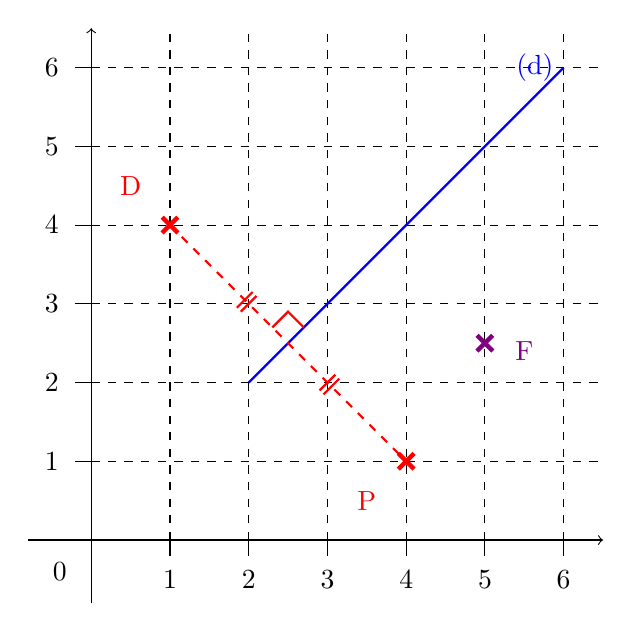
\begin{tikzpicture}
			\draw[dashed] (0,0) grid (6.5,6.5);
			\draw[->] (-0.8,0) -- (6.5,0);
			\draw[->] (0,-0.8) -- (0,6.5);
			\node at (-0.4,-0.4) {0};
			\foreach \r in {1,...,6}{
					\draw (\r,0) -- (\r,-0.2);
					\node at (\r,-0.5) {\r};

					\draw (0,\r) -- (-0.2,\r);
					\node at (-0.5,\r) {\r};
				}

			\coordinate (Dpoint) at (1,4);
			\draw[red,ultra thick] (Dpoint) ++(-0.1,-0.1) -- ++(0.2,0.2) ++(-0.2,0) -- ++(0.2,-0.2);
			\node[red] at ([yshift=0.5cm,xshift=-0.5cm] Dpoint) {D};

			\draw[blue,thick] (2,2) -- (6,6) node[anchor=east] {(d)};

			\coordinate (Fpoint) at (5,2.5);
			\draw[violet,ultra thick] (Fpoint) ++(-0.1,-0.1) -- ++(0.2,0.2) ++(-0.2,0) -- ++(0.2,-0.2);
			\node[violet] at ([yshift=-0.1cm,xshift=0.5cm] Fpoint) {F};

			\coordinate (Ppoint) at (4,1);
			\draw[red,dashed,thick] (Dpoint) -- (Ppoint);
			\draw[red,ultra thick] (Ppoint) ++(-0.1,-0.1) -- ++(0.2,0.2) ++(-0.2,0) -- ++(0.2,-0.2);
			\node[red] at ([yshift=-0.5cm,xshift=-0.5cm] Ppoint) {P};
			\draw[red,thick] (2.9,1.9) -- (3.1,2.1);
			\draw[red,thick] (2.95,1.85) -- (3.15,2.05);
			\draw[red,thick] (1.9,2.9) -- (2.1,3.1);
			\draw[red,thick] (1.85,2.95) -- (2.05,3.15);
			\draw[red,thick] (2.3,2.7) -- (2.5,2.9) -- (2.7,2.7);
		\end{tikzpicture}
	\end{center}
\end{frame}

\begin{frame}
	\begin{center}
		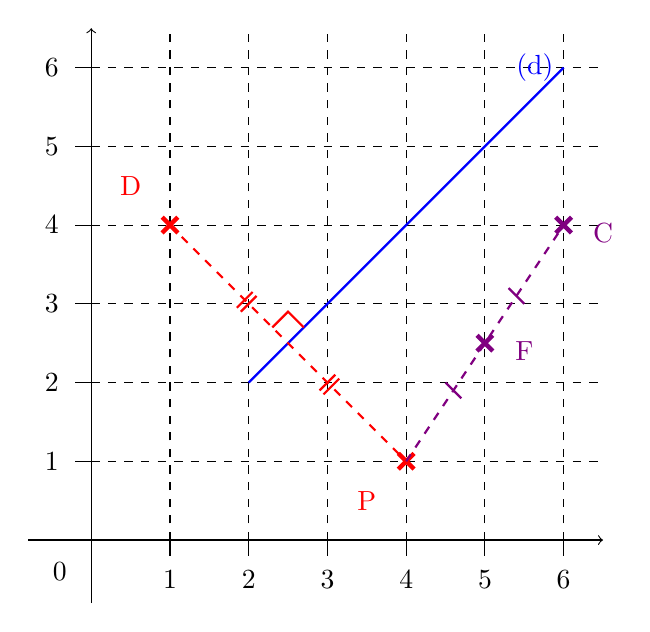
\begin{tikzpicture}
			\draw[dashed] (0,0) grid (6.5,6.5);
			\draw[->] (-0.8,0) -- (6.5,0);
			\draw[->] (0,-0.8) -- (0,6.5);
			\node at (-0.4,-0.4) {0};
			\foreach \r in {1,...,6}{
					\draw (\r,0) -- (\r,-0.2);
					\node at (\r,-0.5) {\r};

					\draw (0,\r) -- (-0.2,\r);
					\node at (-0.5,\r) {\r};
				}

			\coordinate (Dpoint) at (1,4);
			\draw[red,ultra thick] (Dpoint) ++(-0.1,-0.1) -- ++(0.2,0.2) ++(-0.2,0) -- ++(0.2,-0.2);
			\node[red] at ([yshift=0.5cm,xshift=-0.5cm] Dpoint) {D};

			\draw[blue,thick] (2,2) -- (6,6) node[anchor=east] {(d)};

			\coordinate (Fpoint) at (5,2.5);
			\draw[violet,ultra thick] (Fpoint) ++(-0.1,-0.1) -- ++(0.2,0.2) ++(-0.2,0) -- ++(0.2,-0.2);
			\node[violet] at ([yshift=-0.1cm,xshift=0.5cm] Fpoint) {F};

			\coordinate (Ppoint) at (4,1);
			\draw[red,dashed,thick] (Dpoint) -- (Ppoint);
			\draw[red,ultra thick] (Ppoint) ++(-0.1,-0.1) -- ++(0.2,0.2) ++(-0.2,0) -- ++(0.2,-0.2);
			\node[red] at ([yshift=-0.5cm,xshift=-0.5cm] Ppoint) {P};
			\draw[red,thick] (2.9,1.9) -- (3.1,2.1);
			\draw[red,thick] (2.95,1.85) -- (3.15,2.05);
			\draw[red,thick] (1.9,2.9) -- (2.1,3.1);
			\draw[red,thick] (1.85,2.95) -- (2.05,3.15);
			\draw[red,thick] (2.3,2.7) -- (2.5,2.9) -- (2.7,2.7);

			\coordinate (Cpoint) at (6,4);
			\draw[violet,dashed,thick] (Ppoint) -- (Cpoint);
			\draw[violet,ultra thick] (Cpoint) ++(-0.1,-0.1) -- ++(0.2,0.2) ++(-0.2,0) -- ++(0.2,-0.2);
			\node[violet] at ([yshift=-0.1cm,xshift=0.5cm] Cpoint) {C};
			\draw[violet,thick] (4.5,2) -- (4.7,1.8);
			\draw[violet,thick] (5.3,3.2) -- (5.5,3);
		\end{tikzpicture}
	\end{center}
\end{frame}

\begin{frame}
	\begin{center}
		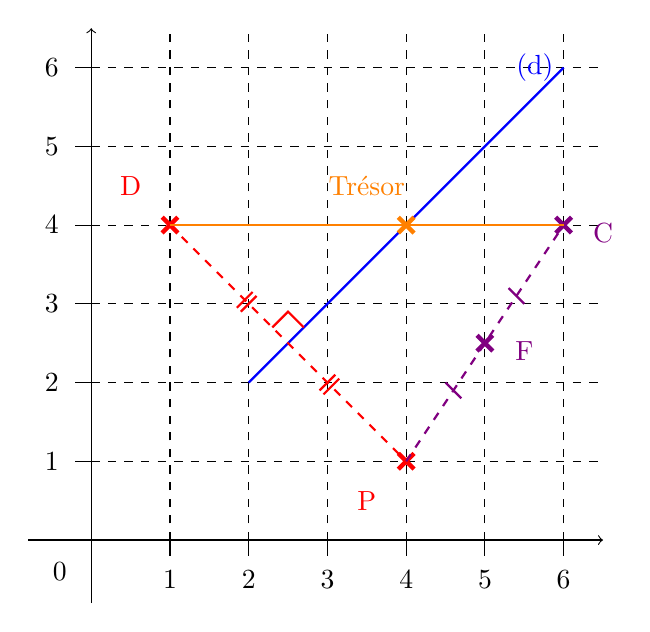
\begin{tikzpicture}
			\draw[dashed] (0,0) grid (6.5,6.5);
			\draw[->] (-0.8,0) -- (6.5,0);
			\draw[->] (0,-0.8) -- (0,6.5);
			\node at (-0.4,-0.4) {0};
			\foreach \r in {1,...,6}{
					\draw (\r,0) -- (\r,-0.2);
					\node at (\r,-0.5) {\r};

					\draw (0,\r) -- (-0.2,\r);
					\node at (-0.5,\r) {\r};
				}

			\coordinate (Dpoint) at (1,4);
			\draw[red,ultra thick] (Dpoint) ++(-0.1,-0.1) -- ++(0.2,0.2) ++(-0.2,0) -- ++(0.2,-0.2);
			\node[red] at ([yshift=0.5cm,xshift=-0.5cm] Dpoint) {D};

			\draw[blue,thick] (2,2) -- (6,6) node[anchor=east] {(d)};

			\coordinate (Fpoint) at (5,2.5);
			\draw[violet,ultra thick] (Fpoint) ++(-0.1,-0.1) -- ++(0.2,0.2) ++(-0.2,0) -- ++(0.2,-0.2);
			\node[violet] at ([yshift=-0.1cm,xshift=0.5cm] Fpoint) {F};

			\coordinate (Ppoint) at (4,1);
			\draw[red,dashed,thick] (Dpoint) -- (Ppoint);
			\draw[red,ultra thick] (Ppoint) ++(-0.1,-0.1) -- ++(0.2,0.2) ++(-0.2,0) -- ++(0.2,-0.2);
			\node[red] at ([yshift=-0.5cm,xshift=-0.5cm] Ppoint) {P};
			\draw[red,thick] (2.9,1.9) -- (3.1,2.1);
			\draw[red,thick] (2.95,1.85) -- (3.15,2.05);
			\draw[red,thick] (1.9,2.9) -- (2.1,3.1);
			\draw[red,thick] (1.85,2.95) -- (2.05,3.15);
			\draw[red,thick] (2.3,2.7) -- (2.5,2.9) -- (2.7,2.7);

			\coordinate (Cpoint) at (6,4);
			\draw[violet,dashed,thick] (Ppoint) -- (Cpoint);
			\draw[violet,ultra thick] (Cpoint) ++(-0.1,-0.1) -- ++(0.2,0.2) ++(-0.2,0) -- ++(0.2,-0.2);
			\node[violet] at ([yshift=-0.1cm,xshift=0.5cm] Cpoint) {C};
			\draw[violet,thick] (4.5,2) -- (4.7,1.8);
			\draw[violet,thick] (5.3,3.2) -- (5.5,3);

			\coordinate (Treasure) at (4,4);
			\draw[orange,thick] (Dpoint) -- (Cpoint);
			\draw[orange,ultra thick] (Treasure) ++(-0.1,-0.1) -- ++(0.2,0.2) ++(-0.2,0) -- ++(0.2,-0.2);
			\node[orange] at ([yshift=0.5cm,xshift=-0.5cm] Treasure) {Trésor};
		\end{tikzpicture}
	\end{center}
\end{frame}

\end{document}